\documentclass[10pt, margin=0.1in]{standalone}

\usepackage{braket}
\usepackage[compat=0.4]{yquant}
\useyquantlanguage{groups}
\usetikzlibrary{quotes, fit}

\begin{document}

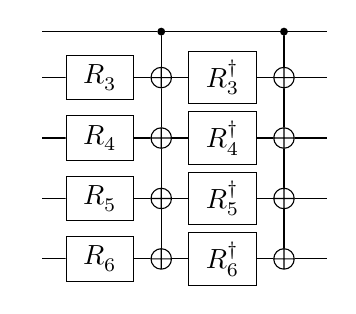
\begin{tikzpicture}
    \begin{yquant*}[loc/.style={style=blue, control style=blue}, nloc/.style={style=red, control style=red}]
    [drawing mode=quality]
    % registers
    qubit {$ $} q[5];
    
    hspace {2mm} -;
    % h q[0];
    box {$\ R_3^{\ }\ $} q[1];
    box {$\ R_4^{\ }\ $} q[2];
    box {$\ R_5^{\ }\ $} q[3];
    box {$\ R_6^{\ }\  $} q[4];
    
    cnot q[1,2,3,4] | q[0];
    box {$\ R_3^\dagger\ $} q[1];
    box {$\ R_4^\dagger\ $} q[2];
    box {$\ R_5^\dagger\ $} q[3];
    box {$\ R_6^\dagger\ $} q[4];
    cnot q[1,2,3,4] | q[0];

    
    % box {$R_{\The\numexpr\idx+2}$} q[1,2,3,4] | q[0];
    
    % hspace {2mm} -;
    % h q[1];
    % box {$R_{\The\numexpr\idx+2}$} q[2,3] | q[1];

    % hspace {2mm} -;
    % h q[2];
    % box {$R_{\The\numexpr\idx+2}$} q[3] | q[2];

    % hspace {2mm} -;
    % h q[3];
    hspace {2mm} -;

    \end{yquant*}
%     \node[fit=(left-0) (left-3) (right-0) (right-3),
% draw, inner sep=6pt, "reversed c-\textsc{not}"] {};
\end{tikzpicture}

\end{document}

